\documentclass[10pt,showpacs,preprintnumbers,footinbib,amsmath,amssymb,aps,prl,twocolumn,groupedaddress,superscriptaddress,showkeys]{revtex4-1}
\usepackage{graphicx}
\usepackage{dcolumn}
\usepackage{bm}
\usepackage[colorlinks=true,urlcolor=blue,citecolor=blue]{hyperref}
\usepackage{color}
\usepackage{listings}
\usepackage{amsmath}
\usepackage{subcaption}
\usepackage{hyperref}
\usepackage{fancyref}
\usepackage{verbatim}
\usepackage{pgfplots}
\pgfplotsset{compat=1.14}
\usepackage{float}

\begin{document}



\title[CPP2]{Computational Physics Project 4\\
\large{Studies of phase transitions in magnetic systems}}

\author{Marc K. Pestana}
\affiliation{Institute of Theoretical Astrophysics, University of Oslo}

\begin{abstract}
The goal of this project is to study Ising model in two dimensions using the Metropolis algorithm implemented as a C++ program to simulate phase transitions. In this program, I modeled the behavior of an idealized two dimensional lattice of spin states, each spin with two states being up or down with corresponding values of $1$ and $-1$. This is called binary system since the objects at each lattice site can only take these two values. For this study, the system was treated as a canonical ensemble since matter are neither added or removed, but energy can be added or removed via a magnetic field or changes in temperature. However, for this study the magnetic field was set to zero so that only temperature variations were studied. At any instant of time, the spin states for the entire lattice take on a particular configuration or arrangements of spin states. We assumed that we had a ferromagnetic ordering, viz $J > 0$.  We used periodic boundary conditions and the Metropolis algorithm. 
I found that at a given critical temperature, my model exhibited a phase transition from a magnetic phase (a system with a finite magnetic moment) to a phase with zero magnetization. We also look at phase transitions and find out that at $J = 1$, $k_B = 1$, there is a phase transition at $T_C = 2.269$, but I only managed to get my approximation of $T_C = 2.283$.
\end{abstract}

\maketitle

\section{Introduction.}
The \href{https://en.wikipedia.org/wiki/Ising_model}{Ising model} has been extremely popular, with applications spanning from studies of phase transitions to simulations in statistics. In one and two dimensions its has analytical solutions for several expectation values and it gives a qualitatively  good understanding of several types of phase transitions.

\section{Theoretical Models}
\paragraph{Summary of Ising model}
In its simplest form the expression for energy in the Ising model, with an externally applied magnetic field, has the form\newline
\newline
\[
E = -J\sum_{<kl>}^{N} s_ls_k - B\sum_{k}^{N} s_k\newline
\]
with $s_k = �1$, N is the total number of spins, J is a coupling constant expressing
the strength of the interaction between neighboring spins, and B is an external
magnetic field interacting with the magnetic moment set up by the spins. However, for this study I assumed that B=0. The symbol $< kl >$ indicates that the sum is over nearest neighbors only. Notice that for $J > 0$ 0 it is energetically favorable for neighboring spins to be aligned. This is consistent the tendency for canonical systems to "seek" the lowest energy state. It is energetically favorable for neighboring spins to be aligned, since alignment means that $s_ks_l  > 0$. This plus  $J>0 \Rightarrow E < 0$ and thus a lower energy state. 
At low enough temperatures, this feature leads to a cooperative phenomenon called spontaneous magnetization. Thus, a given magnetic moment can influence the alignment of spins that are separated from the given spin by a macroscopic distance by propagation through interactions between nearest neighbors. These long range correlations between spins are associated with a long-range order in which the lattice has a net magnetization in the absence of a magnetic field.
\paragraph{Boltzmann distribution}
In order to calculate expectation values such as the mean energy $\langle E \rangle$ or magnetization $\langle M \rangle$ in statistical physics at a given temperature, I used a probability distribution called the Boltzmann distribution\newline
\newline
$P_i(\beta) = \frac{e^{-\beta E_i}}{Z}$\newline
\newline
with $\beta = 1/kT$ being the inverse temperature, $k$ the Boltzmann constant, $E_i$ is the energy of a state $i$ while $Z$ is the partition function for the canonical ensemble defined as
\[
Z = \sum_{i=1}^{M} e^{-\beta E_i}
\]
where the sum extends over all $M$ microstates . $Z$ is the normalization constant for $P_i$ so that it expresses the probability of finding the system in a given configuration enumerated by $i$.
\paragraph{Energy and Magnetization for a specific configuration}
The energy for a specific configuration the energy $E_i$ and magnetization $M_i$ for each $i$, are given by
\[
E_i = -J\sum_{<kl>}^{N} s_ls_k
\]
\[
M_i = sum_{1}^{N} s_i
\]
\paragraph{Configurations}
To better understand what is meant by a configuration, consider first the case
of the one-dimensional Ising model with $B = 0$. In general, a given configuration of N spins in one dimension may look like
\[
\begin{bmatrix}
\uparrow & \uparrow  & \uparrow & \cdots & \uparrow & \downarrow & \uparrow & \cdots & \uparrow  & \uparrow \\
1 & 2 & 3 & \cdots & i - 1 & i & i + 1 & \cdots & N-1 & N\\ 
\end{bmatrix}
\]
In order to illustrate these features let us further specialize to just two spins.
With two spins, since each spin takes two values only, we have 2
2 = 4 possible arrangements of the two spins. These four possibilities are\newline
1 =$\uparrow  \uparrow$ 2 =$\uparrow  \downarrow$ 3 =$\downarrow  \uparrow$ 4 =$\downarrow  \downarrow$ \newline
\paragraph{Boundary conditions}
What is the energy of each of these configurations?
For small systems, I assumed that the interaction between the ends of the configuration matters. Two cases are often used. In the first case one can employ what is called free ends. In systems with large numbers of elements, the ends contribute a small effect on the entire system. However, since I studied small systems, I used so-called Periodic boundary conditions throughout. This means that the
neighbor to the right of $s_N$ is assumed to take the value of $s_1$. Similarly, the
neighbor to the left of $s_1$ takes the value $s_N$ . In this case the energy for the
one-dimensional lattice 2 x 2 lattice becomes
\begin{align*}
E_i &= -J*(s_1s_2 + s_2s_1) \\
\intertext{For each $i$ we obtain each $E_i$ as follows:} \\
E1 &= E_{\uparrow \uparrow} = -2J \\
E2 &= E_{\uparrow \downarrow} = +2J \\
E3 &= E_{\downarrow \uparrow} = +2J \\
E4 &= E_{\downarrow \downarrow} = -2J \\
\end{align*}

For a system described by the canonical ensemble, the energy is an expectation
value since we allow energy to be exchanged with the surroundings (a heat bath
with temperature T) and the number of micro-states is typically large.
I calculated the mean energy and magnetization using the Boltzmann probability distribution $P_i$ as follows:
\begin{align*}
\langle E \rangle &=  \frac{1}{Z} \sum_{i=1}^{M} E_i e^{\beta E_i} \\
\langle M \rangle &=  \frac{1}{Z} \sum_{i=1}^{M} |M_i| e^{\beta E_i} \\
\end{align*}
\paragraph{Energy and specific heat in the canonical ensemble}
The corresponding variance is defined as
\begin{align*}
{{\sigma}_E}^2 &= \langle E^2 \rangle - {\langle E \rangle}^2 \\
&= \frac{1}{Z} \sum_{i=1}^{M} {E_i}^2 e^{\beta E_i} - (\frac{1}{Z} \sum_{i=1}^{M} E_i e^{\beta E_i})^2
\end{align*}
If we divide the latter quantity with $kT^2$ we obtain the specific heat at constant
volume. 
\[
C_V = \frac{1}{k_B T^2}(\langle  E^2 \rangle - {\langle  E  \rangle}^2)
\]
which again can be related to the second derivative of Helmholtz free energy.
\paragraph{Magnetic moments and susceptibility in the canonical ensemble}
Using the same prescription, I computed the mean of the absolute value of the magnetic moment
with the following formula, again using the Boltzmann distribution:
\begin{align*}
\langle M \rangle &= \sum_{i}^{M} | M_i | P_i(\beta) \\
&= \frac{1}{Z} \sum_{i}^{M} | M_i | e^{-\beta E_i} \\
\intertext{and the corresponding variance} \\
{{\sigma}_M}^2 &= \langle M^2 \rangle - {\langle M \rangle}^2 \\
&= \frac{1}{Z} \sum_{i=1}^{M} {M_i}^2 e^{\beta E_i} - (\frac{1}{Z}  \sum_{i=1}^{M} | M_i | e^{\beta E_i})^2 \\
\intertext{This quantity defines also the susceptibility $\chi$ which I used to calculate $\chi$:} \\
chi &= \frac{1}{k_B T^2}(\langle  M^2 \rangle - {\langle  M  \rangle}^2) 
\end{align*}
\section{The Metropolis Algorithm}
The Metropolis algorithm is summarized as follows.
In a calculation of the Ising model in two dimensions, the number of configurations
is given by $2^N$ where $N = L^2$ the number of spins for a lattice of length L.
Fortunately, the Metropolis algorithm considers only ratios between probabilities
and we do not need to compute the partition function at all. The algorithm goes
as follows: \newline
\begin{enumerate}
\item Establish an initial state for the configuration with energy E by creating a random or ordered configuration of the spin states for the lattice.
\item Change the initial configuration by flipping e.g., one spin only. Compute
the energy of this trial state $E_t$.
\item Calculate $\delta E = E_t - E_b$.
\item If $\delta E<0$ we accept the new configuration, meaning that the energy is
lowered and we are hopefully moving towards the energy minimum at a
given temperature. Go to step 7.
\item If $\delta E > 0$, calculate $w = e^{\beta T}$
\item Compare w with a random number $r$ selected using a uniform distribution over $[0,1]$. If $r < w$, then accept the new
configuration, else we keep the old configuration.
\item The next step is to update various expectations values.
\item The steps (2)-(7) are then repeated in order to obtain a sufficently good
representation of states.
\end{enumerate}
Each sweep through the lattice (i.e. when you have summed over
all the spins in a configuration) constitutes what is called a Monte Carlo cycle (MC cycle). One sweep through the lattice is called a cycle or a measurement. To normalize my measurements, I divided the
various expectation values with the total number of cycles. With one acception in part a) and b), I choose to divide by the number of spins to obtain the mean energy as an intensive property of the lattice. In this setting, the energy is now
the energy per spin.

\paragraph{Studies of phase transitions.}
Near $T_C$ we can characterize the behavior of many physical quantities
by a power law behavior. As an example, for the Ising class of models, 
the mean magnetization is given by
\[
  \langle M(T) \rangle \sim \left(T-T_C\right)^{\beta},
\]
where $\beta=1/8$ is a so-called critical exponent. A similar relation
applies to the heat capacity

\[
  C_V(T) \sim \left|T_C-T\right|^{\alpha},
\]
and the susceptibility
\begin{equation}
  \chi(T) \sim \left|T_C-T\right|^{\gamma},
\end{equation}
with $\alpha = 0$ and $\gamma = 7/4$.
Another important quantity is the correlation length, which is expected
to be of the order of the lattice spacing for $T>> T_C$. Because the spins
become more and more correlated as $T$ approaches $T_C$, the correlation
length increases as we get closer to the critical temperature. The divergent
behavior of $\xi$ near $T_C$ is
\begin{equation}
  \xi(T) \sim \left|T_C-T\right|^{-\nu}.
  \label{eq:xi}
\end{equation}
A second-order phase transition is characterized by a correlation length which spans the whole system.
Since we are always limited to a finite lattice, $\xi$ will be proportional with the size of the lattice.  Through so-called finite size scaling relations it is possible to relate the behavior at finite lattices with the results for an infinitely large lattice. The critical temperature in this case scales as

\begin{equation}
 T_C(L)-T_C(L=\infty) = aL^{-1/\nu},
 \label{eq:tc}
\end{equation}
with  $a$ a constant and  $\nu$ defined in Eq. (\ref{eq:xi}).
We set $T=T_C$ and obtain a mean magnetisation

\begin{equation}
  \langle {\cal M}(T) \rangle \sim \left(T-T_C\right)^{\beta}
  \rightarrow L^{-\beta/\nu},
  \label{eq:scale1}
\end{equation}
a heat capacity

\begin{equation}
  C_V(T) \sim \left|T_C-T\right|^{-\gamma} \rightarrow L^{\alpha/\nu},
  \label{eq:scale2}
\end{equation}
and susceptibility

\begin{equation}
  \chi(T) \sim \left|T_C-T\right|^{-\alpha} \rightarrow L^{\gamma/\nu}.
  \label{eq:scale3}
\end{equation}

\section{Case Studies and their Methods}

\paragraph{Case 1, project 4a): For case 1, I studied a simple $2 \times 2$ lattice, and compute analytical expressions for various expectation values.}
I assumed that I had only two spins in each dimension, that is $L=2$. That is I modeled a two dimensional lattice consisting of 4 spins with a total of $4^2 = 16$ states. I found the analytical expression for the partition function, the expectations values for the energy $E$, the mean magnetization $\langle M \rangle$, the specific heat $C_V$ and the susceptibility $\chi$ 
as functions of $T$ using periodic boundary conditions. I used these results as benchmark calculations as a test of the functionality of my software. To perform the computation of the partition function, I first computed the energy for each configuration of the 2 x 2 lattice. I assumed the following scaled values for the constants: $J=1$ (coupling constant) and $k=1$ (for the Boltzmann's constant). 
I also assumed that the nearest neighbors implies that $s_l$ and $s_k$ take on the values both combinations from the set $\{i,i+1\}$. Therefore, the general expression for each configuration is:\newline
 \[
E_i = -J\sum_{<kl>}^{N} s_ls_k
\]
\[
= s_1s_2 + s_2s_1 + s_2s_3 + s_3s_2 + s_3s_4 + s_4s_3 + s_4s_1 + s_1s_4
\]
This formula is computed for all 16 configurations. Each configuration is summarized in a 2 x 2 matrix of up and down arrows. Each term in the energy is determined as follows:\newline
Starting with the upper left element and going clockwise add a term in the energy equation using periodic boundary conditions.
All spins are either up or down. An up spin is given the value $+1$, and a down spin is given the value $-1$.
\paragraph{computing the Energy and Magnetization for each configuration}
The configurations are organized into permutations of like spin combinations (all up, all down, 1 up and 3 down and its complement, 2 up and 2 down).
\paragraph{A spins up or all spins down}
\[
\begin{bmatrix}
\uparrow & \uparrow  \\
\uparrow & \uparrow  \\ 
\end{bmatrix}
or
\begin{bmatrix}
\downarrow & \downarrow  \\
\downarrow & \downarrow  \\ 
\end{bmatrix}
\]
$2$ x $4 \choose 4$ $= 2$\newline
\begin{align*}
E_1 &= -J \times 8 \times (1)(1)&=-8 \\
E_2 &=  -J \times 8 \times (-1)(-1)&=-8 \\
M_1 &=  4 \times +1 &= +4 \\
M_2 &=  4 \times -1 &= -4 \\
\end{align*}
\paragraph{I spin down, 3 spins up}
$4 \choose 1$ $=4$
\[
\begin{bmatrix}
\downarrow & \uparrow  \\
\uparrow & \uparrow  \\ 
\end{bmatrix}
or
\begin{bmatrix}
\uparrow & \downarrow  \\
\uparrow & \uparrow  \\ 
\end{bmatrix}
or
\begin{bmatrix}
\uparrow & \uparrow  \\
\uparrow & \downarrow  \\ 
\end{bmatrix}
or
\begin{bmatrix}
\uparrow & \uparrow  \\
\downarrow & \uparrow  \\ 
\end{bmatrix}
\]
\small
\begin{align*}
E_3 &= -J(2(-1)(1) + 2(1)(1) + 2(1)(1) + 2(1)(-1)) &= 0 \\
E_4 &= -J(2(1)(-1) + 2(-1)(1) + 2(1)(1) + 2(1)(-1)) &= 0 \\
E_5 &= -J(2(1)(1) + 2(1)(-1) + 2(-1)(1) + 2(1)(1)) &= 0 \\
E_6 &= -J(2(1)(1) + 2(1)(1) + 2(1)(-1) + 2(-1)(1)) &= 0 \\
M_3 &= -1 + 3*1 &= 2 \\ 
M_4 &= -1 + 3*1 &= 2 \\
M_5 &= -1 + 3*1 &= 2 \\
M_6 &= -1 + 3*1 &= 2 \\
\end{align*}
\normalsize

\paragraph{3 spin down, 1 spins up}
$4 \choose 3$ $=4$
\[
\begin{bmatrix}
\uparrow & \downarrow  \\
\downarrow & \downarrow  \\ 
\end{bmatrix}
or
\begin{bmatrix}
\downarrow & \uparrow  \\
\downarrow & \downarrow  \\ 
\end{bmatrix}
or
\begin{bmatrix}
\downarrow & \downarrow  \\
\uparrow & \downarrow  \\ 
\end{bmatrix}
or
\begin{bmatrix}
\downarrow & \downarrow  \\
\downarrow & \uparrow  \\ 
\end{bmatrix}
\]
\footnotesize
\begin{align*}
E_7 &= -(2(1)(-1) + 2(-1)(-1) + 2(-1)(-1) + 2(-1)(1)) &= 0 \\
E_8 &= -(2(1)(-1) + 2(-1)(1) + 2(1)(1) + 2(1)(-1)) &= 0 \\
E_9 &= -(2(1)(1) + 2(1)(-1) + 2(-1)(1) + 2(1)(1)) &= 0 \\
E_{10} &= -(2(1)(1) + 2(1)(1) + 2(1)(-1) + 2(-1)(1)) &= 0  \\
M_3 &= +1 + 3*(-1) &= -2  \\
M_4 &= +1 + 3*(-1) &= -2  \\
M_5 &= +1 + 3*(-1) &= -2 \\
M_6 &= +1 + 3*(-1) &= -2 \\
\end{align*}
\normalsize
\newline
\paragraph{2 spins up, 2 spins down $\equiv$ 2 spins down, 2 spins up}
$4 \choose 2$ $=6$\newline
Two configurations with alternating states corresponding to maximum disorder, high temperature, and highest energy
\[
\begin{bmatrix}
\uparrow & \downarrow  \\
\downarrow & \uparrow  \\ 
\end{bmatrix}
or
\begin{bmatrix}
\downarrow & \uparrow  \\
\uparrow & \downarrow  \\ 
\end{bmatrix}
\]
\small
\begin{align*}
E_11 &= -(2(1)(-1) + 2(-1)(1) + 2(1)(-1) + 2(-1)(1))&=8 \\
E_12 &= -(2(-1)(1) + 2(1)(-1) + 2(-1)(1) + 2(1)(-1))&=8 \\
M_11 &= 2(1) + 2(-1) &= 0\\
M_12 &= 2(-1) + 2(1) &= 0\\
\end{align*}
\paragraph{Four configurations with paired alternating states} 
\normalsize
\[
\begin{bmatrix}
\uparrow & \uparrow  \\
\downarrow & \downarrow  \\ 
\end{bmatrix}
or
\begin{bmatrix}
\downarrow & \downarrow  \\
\uparrow & \uparrow  \\ 
\end{bmatrix}
or
\begin{bmatrix}
\uparrow & \downarrow  \\
\uparrow & \downarrow  \\ 
\end{bmatrix}
or
\begin{bmatrix}
\downarrow & \uparrow  \\
 \downarrow & \uparrow  \\ 
\end{bmatrix}
\]
\small
\begin{align*}
E_{13} &= -(2(1)(1) + 2(1)(-1) + 2(-1)(-1) + 2(-1)(1))&=0\\
E_{14} &= -(2(-1)(-1) + 2(-1)(1) + 2(1)(1) + 2(1)(-1))&=0\\
E_{15} &= -(2(1)(-1) + 2(-1)(-1) + 2(-1)(1) + 2(1)(1))&=0\\
E_{16} &= -J(2(-1)(1) + 2(1)(1) + 2(1)(-1) + 2(-1)(-1))&=0\\
M_{13} &= 2(1) + 2(-1) &= 0\\
M_{14} &= 2(1) + 2(-1) &= 0\\
M_{15} &= 2(1) + 2(-1) &= 0\\
M_{16} &= 2(1) + 2(-1) &= 0\\
\end{align*}
\normalsize
Using these these values for all possible energy states of the 2 x 2 Lattice, I computed the analytical expressions for the partition function, the expectations values for the energy $E$, the mean magnetization $\langle M \rangle$ , the specific heat $C_V$ and the susceptibility $\chi$ 
as functions of  $T$ using periodic boundary conditions. My calculations and their results can be found below in the results section under case 1, project 4a).

\paragraph{Case 2, project 4b):  For case 2, a C++ program was created implementing the Ising model and the Metropolis algoritm.}
I used the C++ program to compute the mean energy 
$E$, mean magnetization 
$\vert M\vert$, the specific heat $C_V$ and the susceptibility $\chi$ 
as functions of  $T$ using periodic boundary conditions for 
$L=2$ in the $x$ and $y$ directions. 
I compared my results with the expressions from a)
for  a  temperature $T=1.0$ (in units of $kT/J$). The results comparing the exact value to the numerical value can be seen in figure \ref{fig:meanE}, \ref{fig:CV}, \ref{fig:meanM} and \ref{fig:chi}. In these figures, we compare the number of MC cycles to the precision of the numerical approximation as the blue line approaches the green exact value.
I determined the number of Monte Carlo cycles needed in order to achieve a good agreement by repeatedly calling the program, increasing the number of cycles by 1 order of magnitude starting with 100.

\paragraph{Case 3, project 4c): For case 3, determine when the most likely state reached.} For this case, I choose a square lattice with $L=20$ spins in the $x$ and $y$ directions. Using the simulation software, I performed a study of the time, as defined as the number 
of Monte Carlo sweeps of the lattice, needed before my model reached an equilibrium condition 
that allowed me to determine the expectations values for mean energy and mean magnetization. I plotted the various expectations values as functions of the number of Monte Carlo cycles.
Each plot combines data for two temperatures of $T=1.0$ and $T=2.4$ (in units of $kT/J$), and the random and ordered configurations(all spins pointing up). My program reported the number of Monte Carlo cycles needed before you reach an equilibrium condition in figures \ref{fig:meanE}, \ref{fig:CV}, \ref{fig:meanM} and \ref{fig:chi}. I repeated this analysis for $T=2.4$. I estimated, based on these values, an equilibration time (number of MC cycles), and made a plot of the total number of accepted configurations as a function of the total number of Monte Carlo cycles that showed how the number of accepted configurations behaved as function of temperature $T$ (see figure \ref{fig:4c_MC_config}).
In figures \ref{fig:4c_MC_E} and \ref{fig:4c_MC_Mabs} we see expectation values with different initial values converging towards each other. The blue line in all three plots represents an ordered configurations where all the initial spins in the lattice are pointing in the same direction with a temperature $T = 1$. The green line represents a randomized configurations where at $T = 1$. The red and cyan lines represent an ordered and a random configuration respectively at $T = 2.4$.  

\paragraph{Case 4, project 4d): For case 4, I analyzed the probability distribution.}
I computed the probability $P(E)$ for the previous system with $L=20$ and the same temperatures, that is at $T=1.0$ and $T=2.4$. I computed this probability by creating a histogram of energy levels about $.1$ wide. I started the computation after the steady state situation has been reached. Then, I compared my results with the computed variance in energy $\sigma^2_E$ and compared (below in the results section) the behavior I observed.  In figure \ref{fig:4d_T1} and \ref{fig:4d_T2.4} we see the probability distribution of the equilibrium states of $T = 1$ and $T = 2.4$ respectively.

\paragraph{Case 5, project 4e) For case 4, I studied phase transitions in lattices of various sizes.}
I studied the behavior of the Ising model in two dimensions close to the critical temperature as a function of the lattice size $L\times L$. I calculated the expectation values for $\langle E\rangle$ and $\langle \vert M\vert\rangle$, the specific heat
$C_V$ and the susceptibility $\chi$ as functions of $T$ for $L=40$,
$L=60$, $L=80$ and $L=100$ for $T\in [2.0,2.3]$ with a step in
temperature $\Delta T=0.05$ or smaller.

I plotted $\langle E\rangle$, $\langle \vert M\vert\rangle$, $C_V$ and $\chi$ as functions of $T$. I used the rate of change in the expectation values and variances an indication of a phase transition. I used the absolute value $\langle \vert M\vert\rangle$ when I evaluated $\chi$. For these production runs I parallelized the code using MPI. I used optimization flags with the MPI version of the c++ compiler (i.e. mpic++ -O3 -o main.x main.cpp), when compiling. I performed a timing analysis of some selected runs in order to see that you optimized the speedup using the parallelized code.
In figure \ref{fig:4e_E}, \ref{fig:4e_CV}, \ref{fig:4e_Mabs}, \ref{fig:4e_chi}, we see the mean energy, specific heat capacity, mean magnetization and magnetic susceptibility respectively for $L=40$, $L=60$, $L=80$ and $L=100$ lattice sizes. 

\paragraph{Case 6, project 4f): In Case 6, I extracted the critical temperature.}
I used Eq. (\ref{eq:tc}) and the exact result $\nu=1$ in order to estimate $T_C$ in the thermodynamic limit $L\rightarrow \infty$ using my simulations with $L=40$, $L=60$, $L=100$ and $L=140$
The exact result for the critical temperature (\href{{http://journals.aps.org/pr/abstract/10.1103/PhysRev.65.117}}{after Lars Onsager}) is $kT_C/J=2/ln(1+\sqrt{2})\approx 2.269$ with $\nu=1$.

\section{Results}
\paragraph{Case 1, project 4a): For case 1, benchmark calculations for my next steps.} The derivation, and evaluation of and their values for $T=1, J=1$, and $k_b=1$:
\begin{table}[h]
\caption{A summary of spin configurations with energy and magnetic moment}
\begin{tabular}{|l|l|l|l|}
\hline
Number of up-spins & Degeneracy & Energy & Magnetization\\
\hline
4&1&-8J&4\\
\hline
3&4&0&2\\
\hline
2&4&0&0\\
\hline
2&2&8J&0\\
\hline
1&4&0&-2\\
\hline
0&1&-8J&-4\\
\hline
\end{tabular}
\label{tab:energies}
\end{table}
\paragraph{computing the partition function}
\small
\begin{align*}
Z &= \sum_{1}^{16} e^{-\frac{E_i}{kT}}=\sum_{1}^{16} e^{-\frac{E_i}{T}} \\
\intertext{which after inserting the values for $E_i$ above becomes:} \\
Z &= 4 cosh(\frac{8}{T})+12 \\
\intertext{computing the mean energy $\langle E \rangle$} \\
\langle E \rangle &= \frac{\sum_{1}^{16} E_i e^{-E_i/T}}{Z} \\
&= \frac{-16e^{+\frac{8}{T}} + 16e^{-\frac{8}{T}}}{Z} \\
&= \frac{-32(sinh(8/T)}{Z} \\
&= \frac{-8sinh(\frac{8}{T})}{cosh(\frac{8}{T})+3} \\
\intertext{computing the mean square energy $\langle E^2 \rangle$} \\
\langle E^2 \rangle &= \frac{\sum_{1}^{16} E_i^2 e^{-E_i/T}}{Z} \\
&= \frac{128e^{+8/T} + 0 + 0 + 0 + 128e^{-8/T}}{Z} \\
&= 256(cosh(8/T))/(4cosh(8/T)+12) \\
&= 256\frac{cosh(8/T)}{(4cosh(8/T)+12)} \\
&= 64\frac{cosh(8/T)}{(cosh(8/T)+3)} \\
\intertext{computing the mean magnetization} \\
\langle |M| \rangle &= \frac{1}{Z} \sum_{1}^{16} |M_i| e^{-\frac{E_i}{T}} \\
&= 4e^{+8/T}+4(2) + 0 + 0 + 0 + 4(2) + 4e^{+8/T}/Z  \\
&= \frac{(4e^{+8/T} + 4e^{+8/T} + 16)}{Z} \\
&= \frac{(8e^{+8/T} + 16)}{Z} \\
&= \frac{8(e^{+8/T} +2)}{(4cosh(8/T)+12)} \\
&= \frac{2(e^{+8/T} +2)}{(cosh(8/T)+3)} \\
\intertext{computing the mean square magnetization} \\
\langle M^2 \rangle &= \frac{1}{Z} \sum_{1}^{16} M_i^2 e^{-\frac{E_i}{T}} \\
&= 16e^{+8/T}+4(4) + 0 + 0 + 0 + 4(4) + 16e^{+8/T}/Z\\
&= 32e^{+8/T} + 32/Z\\
&= 32e^{+8/T} + 32/(4cosh(8/T)+12)\\
&= 8(e^{+8/T} + 1)/(cosh(8/T)+3) \\
\intertext{computing the Specific Heat at constant volume} \\
C_V &= \frac{1}{k_B T^2}(\langle  E^2 \rangle - {\langle  E  \rangle}^2) \\
&= (\frac{64}{T^2})\frac{(1+3\cosh(8/T))}{(\cosh(8/T)+3)^2} \\
\intertext{computing the magnetic suseptability} \\
\chi &= \frac{1}{k_B T^2}(\langle  M^2 \rangle - {\langle  M  \rangle}^2) \\
&= \frac{1}{k_B T^2}(\frac{8(e^{+8/T} + 1)}{(cosh(8/T)+3)} - (\frac{2(e^{+8/T} +2)}{(cosh(8/T)+3)})^2)\\
\end{align*}
I used the wolfram alpha websites calculator to create the following list of desired values:
\begin{align*}
Z &= 5973.917 \\
\langle E\rangle &= -7.9840 \\
\langle |M|\rangle &= 3.9948 \\
C_V &= 0.1284 \\
\chi &= 0.0160
\end{align*}
Or the values per spin:
\begin{align*}
\frac{\langle E\rangle}{L^2} &= -1.9960\\
\frac{C_V}{L^2}&= 0.0321\\
\frac{\langle |M|\rangle}{L^2} &= 0.9987\\
\frac{\chi}{L^2} &= 0.0040
\end{align*}


 \paragraph{Case 2, project 4b):  For case 2, comparing the C++ code implementing the Ising mode with the analytical results for case 1.}
The number cycles to reach good agreement with the analytical results is approximately $10^7$. The following table compares the analytical values with the computed ones:
\small
\begin{table}[h]
\caption{A comparison of the analytical values for mean energy, mean magnetization, specific heat(at constant volumn), and the magnetic suseptibility.}
\begin{tabular}{l|l|l|l|l|l|}
\hline
Mode & $\langle E \rangle$ & $\langle |M| \rangle$ & $C_v$ & $\chi$ \\
\hline
Analytical & -7.9840 & 3.9948 & 0.1284 & 0.0160 \\
\hline
Monte Carlo & -7.9836 & 3.9946 & 0.1275 & 0.0159 \\
\hline
\end{tabular}
\label{tab:mcvals}
\end{table}

\begin{figure}[H]
\centering
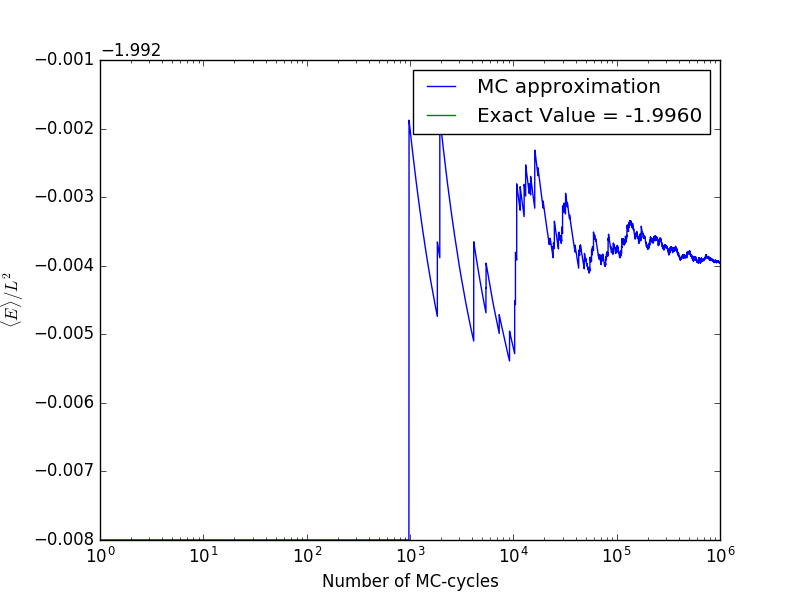
\includegraphics[width=\linewidth]{4b_EMC_vs_exact_log}
\caption{Mean energy per spin squared using Monte-Carlo approximation. We can see the numerical values closing in on the analytcial value after running a lot of cycles.}
\label{fig:meanE}
\end{figure}

\begin{figure}[H]
\centering
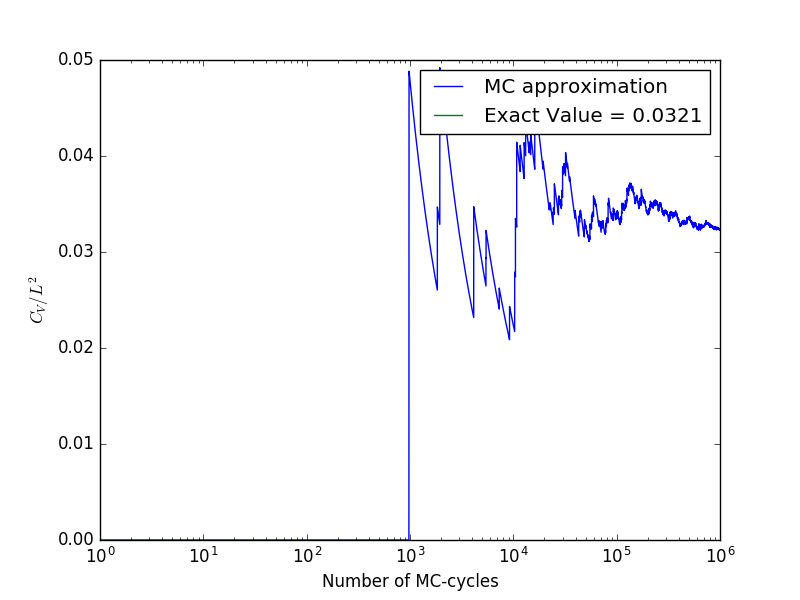
\includegraphics[width=\linewidth]{4b_CVMC_vs_exact_log}
\caption{Specific heat capacity per spin squared using converging Monte-Carlo approximation.}
\label{fig:CV}
\end{figure}

\begin{figure}[H]
\centering
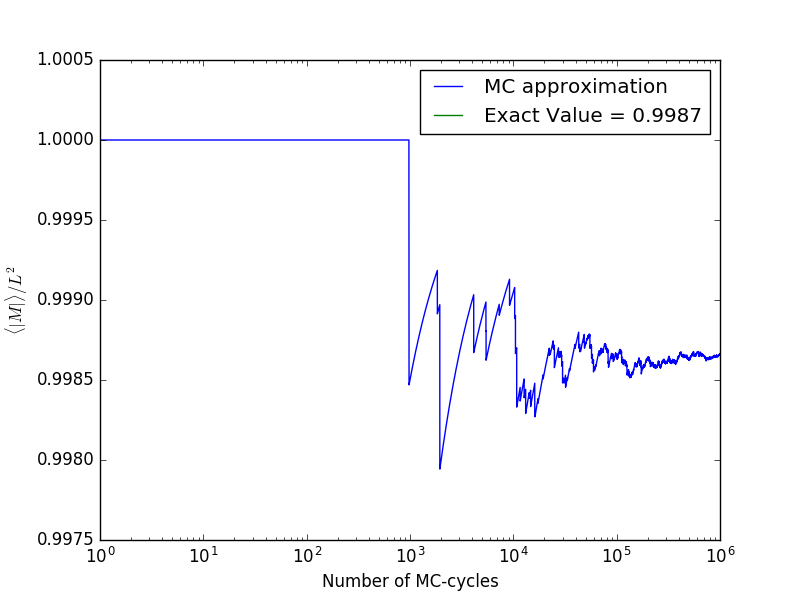
\includegraphics[width=\linewidth]{4b_MMC_vs_exact_log}
\caption{Absolute value of the mean magnetization per spin squared converging using Monte-Carlo approximation.}
\label{fig:meanM}
\end{figure}

\begin{figure}[H]
\centering
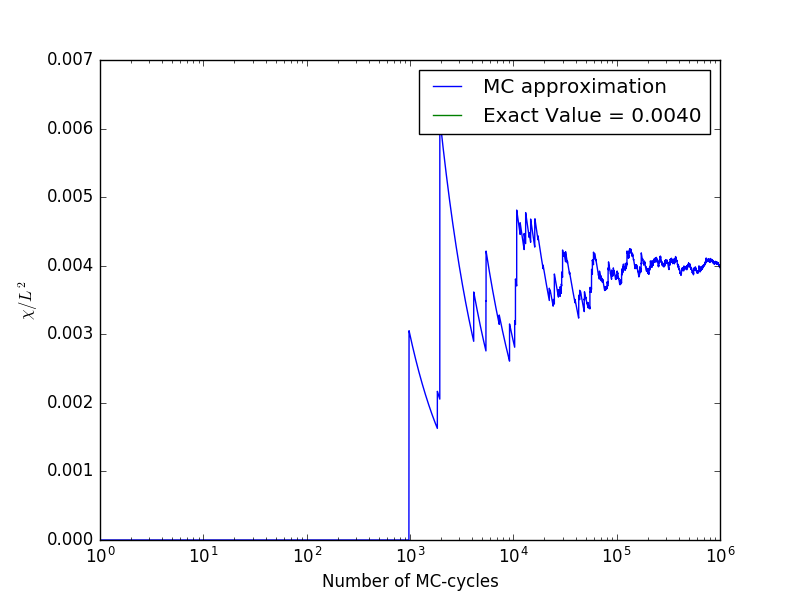
\includegraphics[width=\linewidth]{4b_chiMC_vs_exact_log}
\caption{Magnetic susceptability per spin squared converging using Monte-Carlo approximation.}
\label{fig:chi}
\end{figure}


\paragraph{Case 3, project 4c): For case 4,  expectations values as functions of the number of Monte Carlo cycles.} figure \ref{fig:4c_MC_config} showed how the number of accepted configurations behaved as function of temperature $T$.

\begin{figure}[H]
\centering
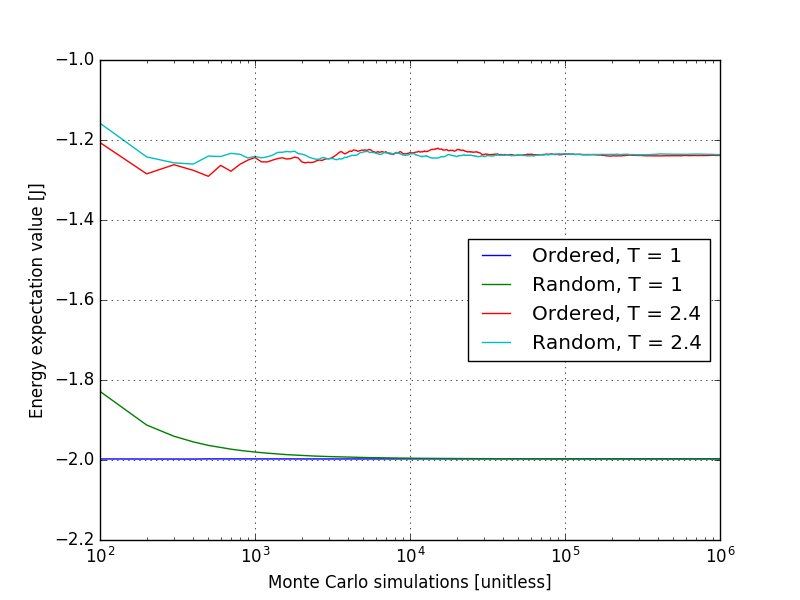
\includegraphics[width=\linewidth]{4c_MC_E}
\caption{Energy expectation value per spin squared as a function of MC-cycles. Different plots for different temperatures and starting lattice orientations.}
\label{fig:4c_MC_E}
\end{figure}

\begin{figure}[H]
\centering
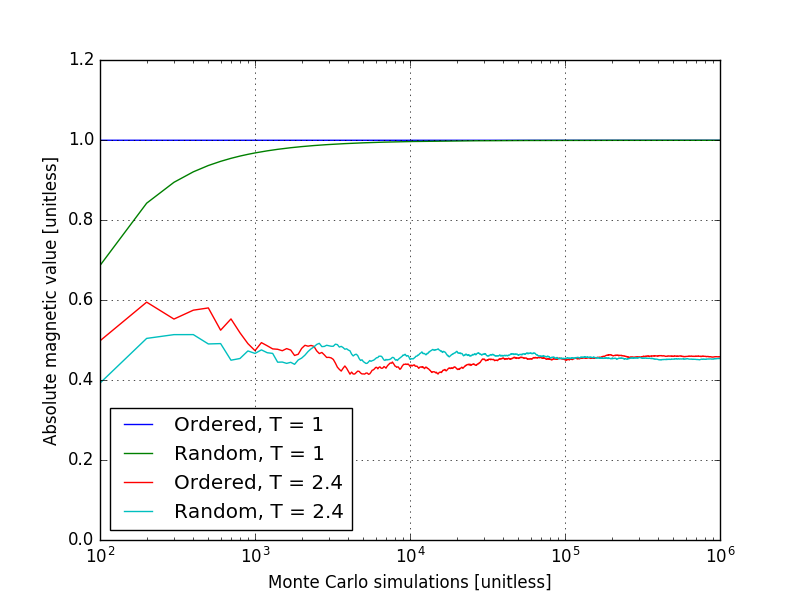
\includegraphics[width=\linewidth]{4c_MC_Mabs}
\caption{Absolute expectation value for magnetic moment as a function of MC-cycles. Different plots for different temperatures and starting lattice orientations.}
\label{fig:4c_MC_Mabs}
\end{figure}

\begin{figure}[H]
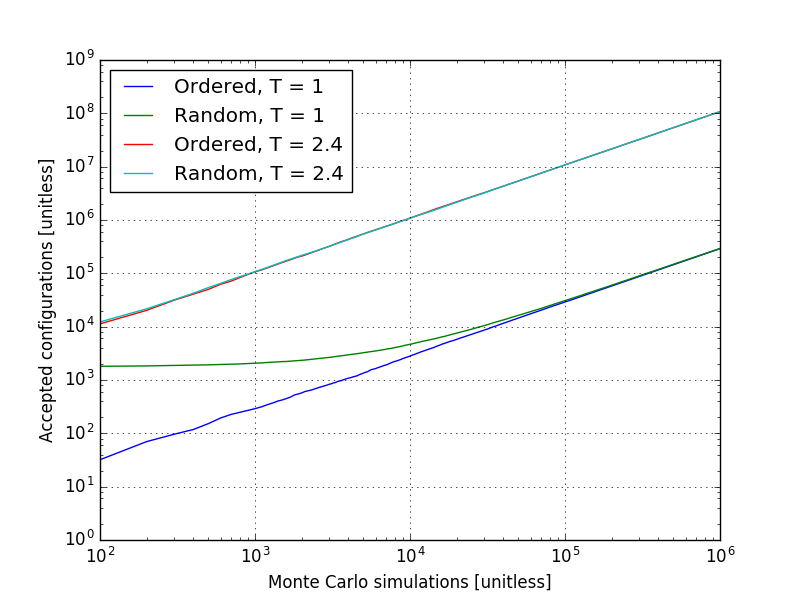
\includegraphics[width=\linewidth]{4c_MC_config}
\caption{Comparison of the number of accepted configurations as a function of MC-cycles. Comparison between a random lattice starting configuration and an ordered starting configuration with all spins starting in the same direction. Different plots for different temperatures and starting lattice orientations.}
\label{fig:4c_MC_config}
\end{figure}


\paragraph{Case 4, project 4d): For case 4, probability distribution.}
In figure \ref{fig:4d_T1} and \ref{fig:4d_T2.4} we see the probability distribution of the equilibrium states of $T = 1$ and $T = 2.4$ respectively. Figure \ref{fig:4c_MC_config} shows us the total number of accepted configurations in our model as a function of MC cycles at each given temperature, with ordered and randomized lattice configurations. 

\begin{figure}[H]
\centering
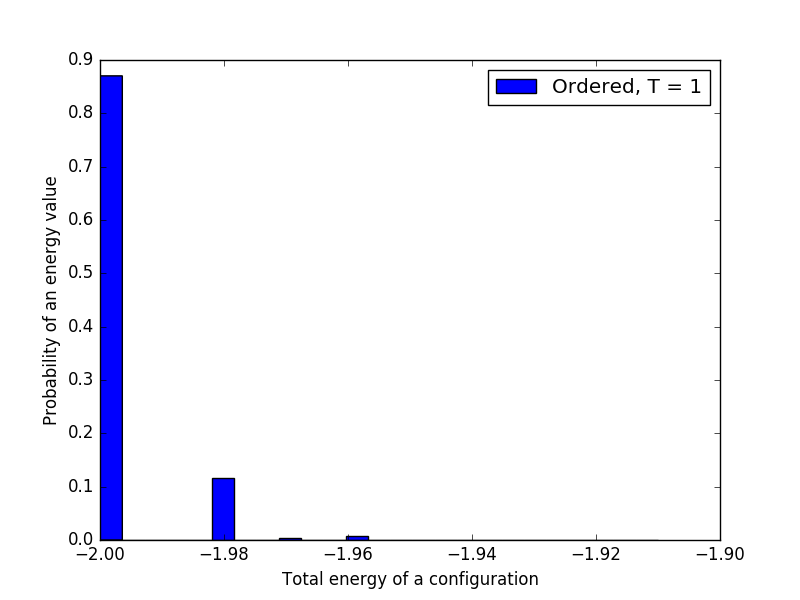
\includegraphics[width=\linewidth]{4d_hist_E_o_1_steady}
\caption{Probability distribution histogram of the equilibrium state for $T= 1$. The plots for the ordered start and the randomized start configuration look exactly the same.}
\label{fig:4d_T1}
\end{figure}

\begin{figure}[H]
\centering
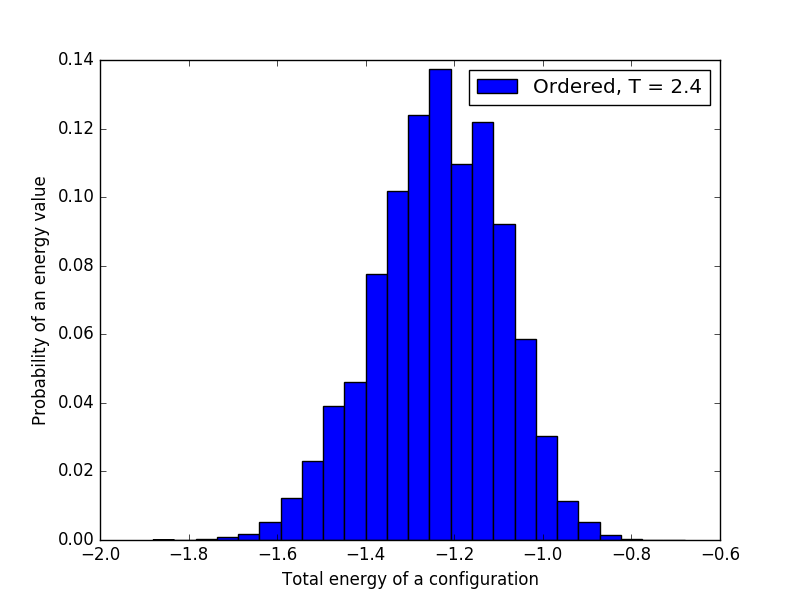
\includegraphics[width=\linewidth]{4d_hist_E_o_2p4_steady}
\caption{Probability distribution histogram of the equilibrium state for $T= 2.4$. The plots for the ordered start and the randomized start configuration look exactly the same.}
\label{fig:4d_T2.4}
\end{figure}


\paragraph{Case 5, project 4e): Case 5, Numerical studies of phase transitions.}

\begin{figure}[H]
\centering
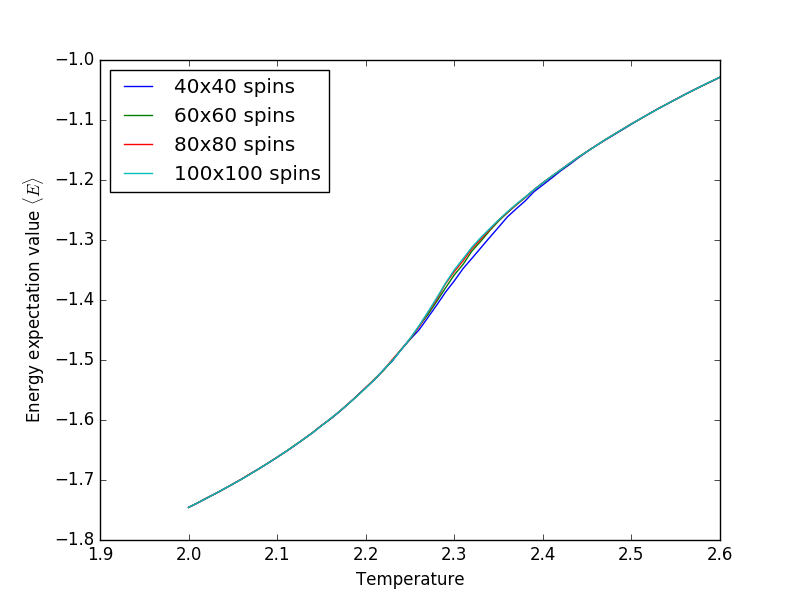
\includegraphics[width=\linewidth]{4e_T_E}
\caption{Numerical approximation to the energy expectation value for $L \in \{40, 60, 80, 100\}$. Notice the phase transition near $T = 2.3$.}
\label{fig:4e_E}
\end{figure}

\begin{figure}[H]
\centering
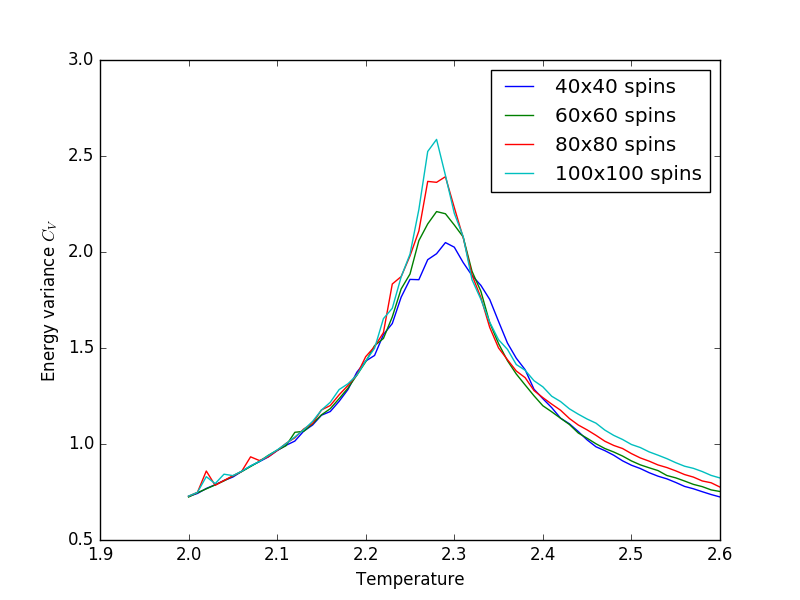
\includegraphics[width=\linewidth]{4e_T_CV}
\caption{Numerical approximation to the specific heat capacity for $L \in \{40, 60, 80, 100\}$. We clearly see the phase transition because of the large variance it causes near $T = 2.3$. }
\label{fig:4e_CV}
\end{figure}

\begin{figure}[H]
\centering
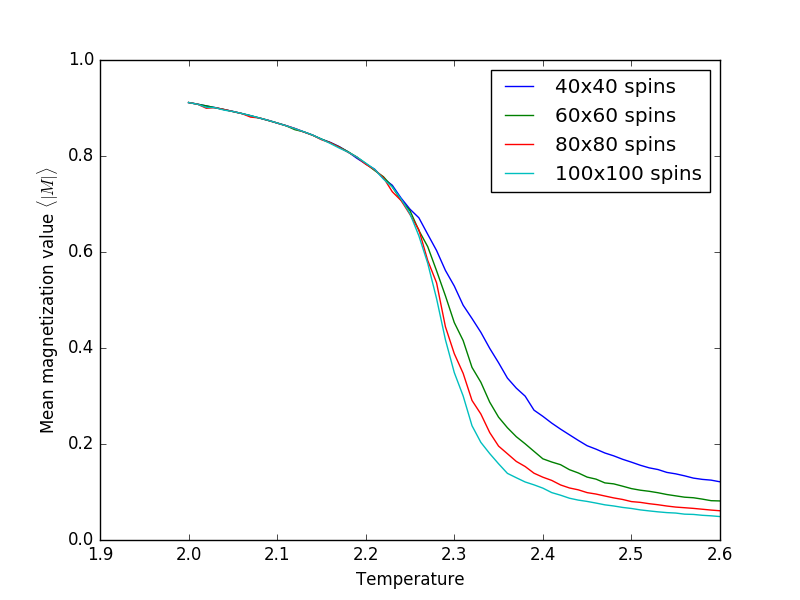
\includegraphics[width=\linewidth]{4e_T_Mabs}
\caption{Numerical approximation to the magnetization expectation value for $L \in \{40, 60, 80, 100\}$. There is a phase transition happening around $T = 2.3$.}
\label{fig:4e_Mabs}
\end{figure}

\begin{figure}[H]
\centering
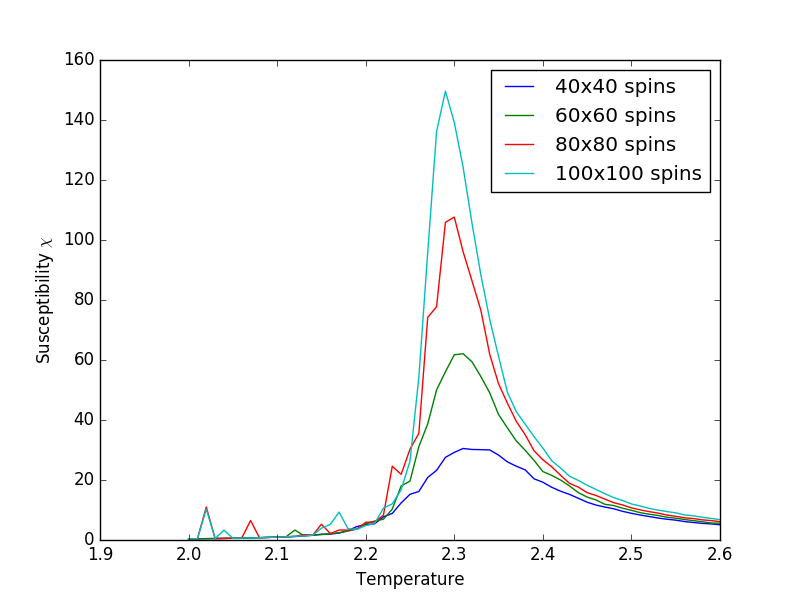
\includegraphics[width=\linewidth]{4e_T_chi}
\caption{Numerical approximation to the magnetic susceptibility for  $L \in \{40, 60, 80, 100\}$. As with figure \ref{fig:4e_CV}, we can clearly see the phase transition happening near $T = 2.3$.}
\label{fig:4e_chi}
\end{figure}

\paragraph{Case 6, project 4f): In Case 6, I extracted the critical temperature.}

\begin{figure}[H]
\centering
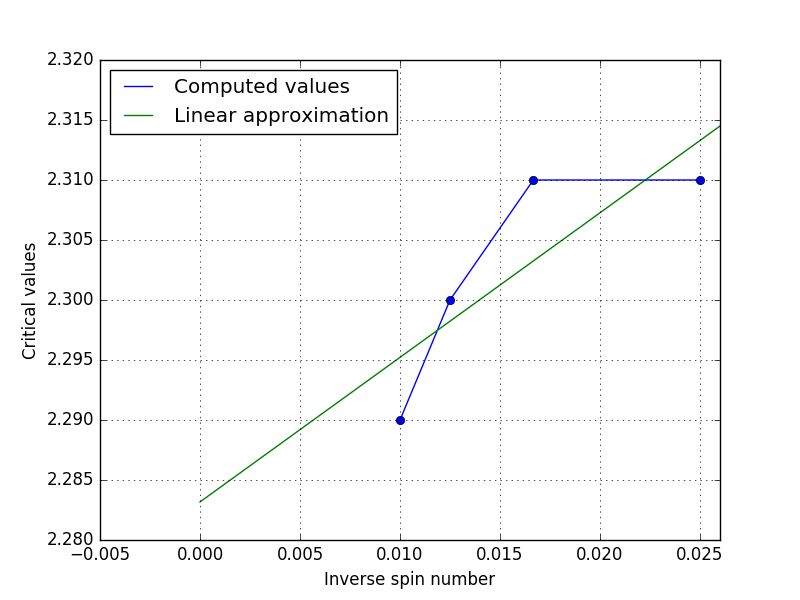
\includegraphics[width=\linewidth]{4f_extrap_blunt}
\caption{Linear extrapolation to approximate $T_C$ when $L\rightarrow\infty$. As we can see, our approximation gives us a critical temperature of $T_C\approx 2.283$.}
\label{fig:4f_sharp}
\end{figure}

Also from figure \ref{fig:4e_chi} we extract the extrema points, which we use to create a linear extrapolation in figure \ref{fig:4f_sharp}. Figure \ref{fig:4f_sharp} is an approximation to the critical temperature $T_C$. We see that the critical temperature at $\frac{1}{L} = 0$, i.e. where $L\rightarrow\infty$, is about $T_C \approx 2.283$ according to our approximations.  

\section{Discussion}
In figures \ref{fig:meanE} to \ref{fig:chi}, we compared the exact values of the energy computed from analytical expressions, magnetic moment, the specific heat capacity and the susceptibility to their respective Monte-Carlo approximations as functions of number of MC-cycles. In these plots we see that the Metropolis algorithm utilizes significant cpu cycles if we want to get a close approximation. To get a relatively good estimate of the exact value we seem to need execcute more than $4\cdot 10^5$ MC cycles. The exact number of cycles we need to run, however, is dependent on the precision we need. If we're only looking to have the graph "stabilize", we need about $2\cdot 10^5$ cycles. 

After about $10^6$ cycles, the algorithm gives accurate results, but larger configurations take more cycles to converge as we only flip one spin every cycle at most. This makes it so that it requires an exponentially increasing number of cycles for a computer to simulate larger systems using this algorithm.

\textbf{Equilibrium}
If we look at figure \ref{fig:4c_MC_E} and \ref{fig:4c_MC_Mabs}, we see that the time to equilibrium is about $10^5$ MC cycles for when the temperature is set to $T = 2.4$. For $T = 1$, the equilibrium time appears to be $10^4$, but only for the random start configuration. This is because when $T = 1$ and we start with a ordered system, the energy is at its lowest state, making it very unlikely for the system to change state to a higher energy state. This is confirmed by figure \ref{fig:4d_T1}, a histogram of the values taken by the system once it reaches its equilibrium state. As you can see, the probability of being in the lowest energy state is higher than the other states due to its low variance. 

When $T = 2.4$, we need about $10^5$ cycles to reach equilibrium. Looking at figure \ref{fig:4d_T2.4}, we can see that the probability distribution for the equilibrium state is different from the low temperature distribution. This is due to its larger variance, which matches up well with the variance we calculated in our exercise. The probability of "jumping" to higher energy states is higher than in the low temperature simulation. 

In figure \ref{fig:4c_MC_config}, we see the difference in number of accepted lattice configurations as a function of MC-cycles. This plot shows that the number of accepted configurations per cycle increases linearly when T = 2.4. This is because the probability of accepting a new configuration is nearly constant the simulation because of the relatively large number of degenerate energy states available to the system because of its high temperature. This also explains the fact that there are more accepted configurations for the higher temperature. For $T = 1$, the random configuration we find more accepted configurations. This is because the probability of this system being in a high energy state is so low that almost all the early lower energy configurations are accepted, compared to the ordered lattice configuration which is almost linear. While the number of configurations is higher on the randomized plot, it hard to detect at large MC cycles because of the logarithmic scale. 


\textbf{Phase Transitions}
Examining figure \ref{fig:4e_E}, we see that the steepest part of the slope is at the phase transition temperature. The reason different lattice sizes show different slopes around this transition is probably because of the large divergence in variance in that area compared to other regions along the line. From our exact result we predict that divergence is greatest at the critical temperature of $T_C = 2.269$. 

From figure \ref{fig:4f_sharp}, however, our approximation was about $T_C = 2.283$. This is probably because we used a small sample of computed correlation points. Also, it might have had something to do with the random number generators used in our implementation of the MC method, however, this is less likely for the lower values of L as we have previously confirmed. Yet, for high accuracy of our algorithms for lower Ls, the number of cycles still is about $10^6$. For the higher values of L some numerical problems persist as the algorithm might need more cycles to reach the same precision. We are certain that if we were to run the algorithm for higher values of L, we would get a better approximation to the exact value if we also increased the number of MC cycle higher than $10^6$. 

We might also have gotten higher accuracy if we used the extrema points from figure \ref{fig:4e_CV} as well as figure \ref{fig:4e_chi} to compute $T_C$. We still manage to get quite close to the exact value, so the result can be considered a success. 

\section{Extra Material}
You can find the project code, plots files, report, and other files at \url{https://github.com/marckp/project4}
\begin{thebibliography}{99}
\bibitem{mhjensen} M. H.~Jensen, Computational Physics 08.11.2017 \url{https://github.com/CompPhysics/ComputationalPhysics/blob/master/doc/Projects/2017/Project4/pdf/Project4.pdf} and\\ Computational~Physics 31.10.2016 \url{https://github.com/CompPhysics/ComputationalPhysics/blob/master/doc/Programs/ParallelizationMPI/IsingModel.cpp}
\bibitem{marius}M. Pram 
\bibitem{espen} E. Hodne
\end{thebibliography}
\end{document}


